\section{Generazione dei mockup}
\subsection{Generazione delle escursioni con \href{https://chat.openai.com/auth/login}{ChatGPT}}\label{sect:genEventi}
Per fornire una dimostrazione del sistema abbiamo caricato nel database una decina di escursioni di esempio.
La generazione di mockup di buona qualità generalmente richiede molto lavoro manuale affinché rispecchino la forma dei dati
che nel mondo reale verranno forniti alla piattaforma. Se si usano, per esempio, stringhe troppo corte o troppo lunghe si rischia di creare
un prodotto non adatto al mondo reale.
Nell'ultimo anno sono emersi numerosi Large Language Model (LLM) che si rivelano molto efficaci nella rielaborazione di testi, specialmente quando gli viene 
fornito un esempio su cui lavorare. Il nostro problema di generazione dei mockup è appunto un'istanza di questo problema che si presta molto bene ad essere
risolta dal un LLM\@.Abbiamo scelto di lavorare con ChatGPT essendo uno dei modelli più accessibili e prestanti al momento disponibili.
Il primo passo è stato elaborare un prompt che istruisse la macchina sul problema che volevamo risolvesse e le fornisse un esempio scritto da noi su cui lavorare (Figura~\ref*{fig:prompt1}).
Abbiamo quindi ricevuto una risposta con alcuni dei mockup richiesti (Figura~\ref*{fig:answ2}).
Avendo verificato che tutti i vincoli venissero rispettati abbiamo chiesto di formulare anche i mockup mancanti per arrivare a 10 (Figura~\ref*{fig:prompt2}).
\subsection{Generazione dei profili utente con \href{https://chat.openai.com/auth/login}{ChatGPT}}
Per gli stessi motivi esplicati in \ref*{sect:genEventi}abbiamo generato anche 4 profili utente: 2 organizzatori e 2 utenti normali (Figura~\ref*{fig:prompt3}).
\newpage
\subsection{Generazione delle immagini delle escursioni con \href{https://www.craiyon.com}{Crayon V3}}
Fornendo il prompt ``A fictitious mountain range in northern Italy'' abbiamo istruito un modello per la generazione di immagini di creare alcune immagini che potessimo creare per arricchire la presentazione dei nostri mockup (Figura~\ref*{fig:prompt4}).
Con la funzione di upscaling abbiamo infine aumentato la qualità delle immagini che più ci piacevano e le abbiamo scaricate. Tutte le immagini selezionate sono disponibili sulla repository del progetto.
\newpage
\begin{figure}[ht]
  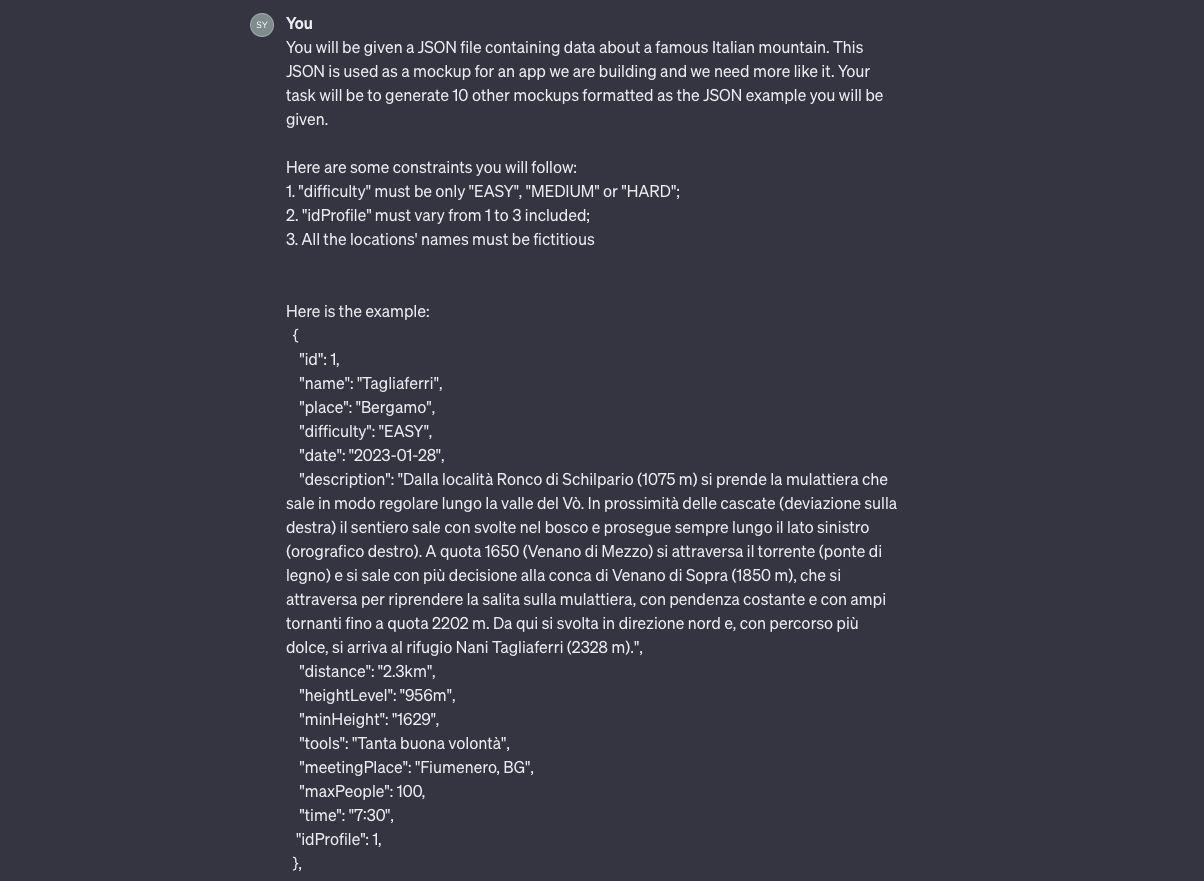
\includegraphics[width=\textwidth]{Iterazione 3/images/prompt1.png}
  \caption{Primo prompt per la generazione di escursioni}\label{fig:prompt1}
\end{figure}
\begin{figure}[ht]
  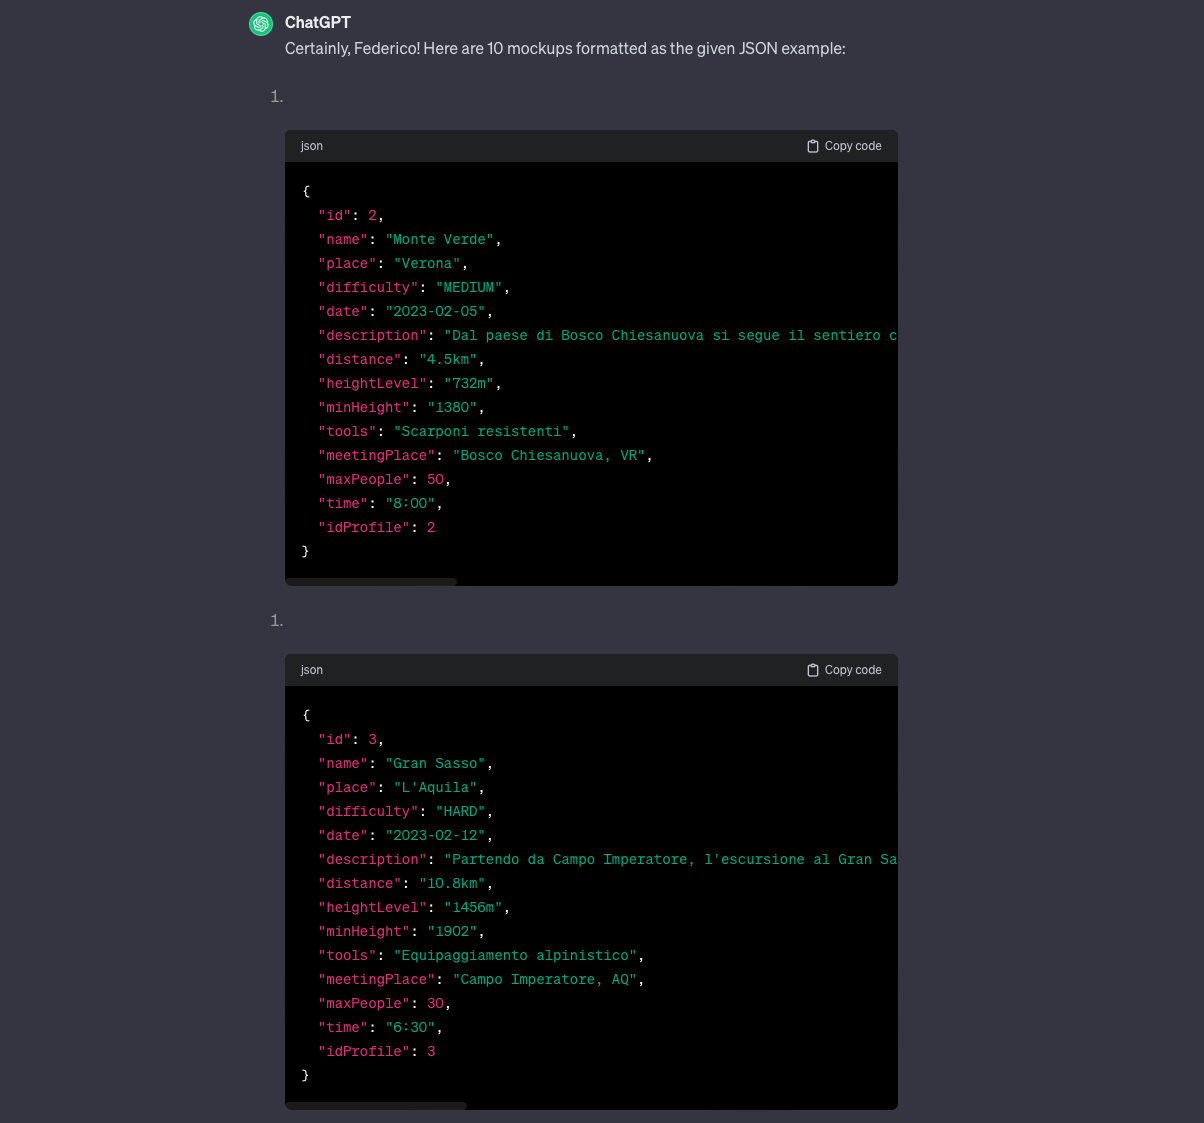
\includegraphics[width=\textwidth]{Iterazione 3/images/answer1.png}
  \caption{Risposta parziale al primo prompt}\label{fig:answ1}
\end{figure}
\begin{figure}[ht]
  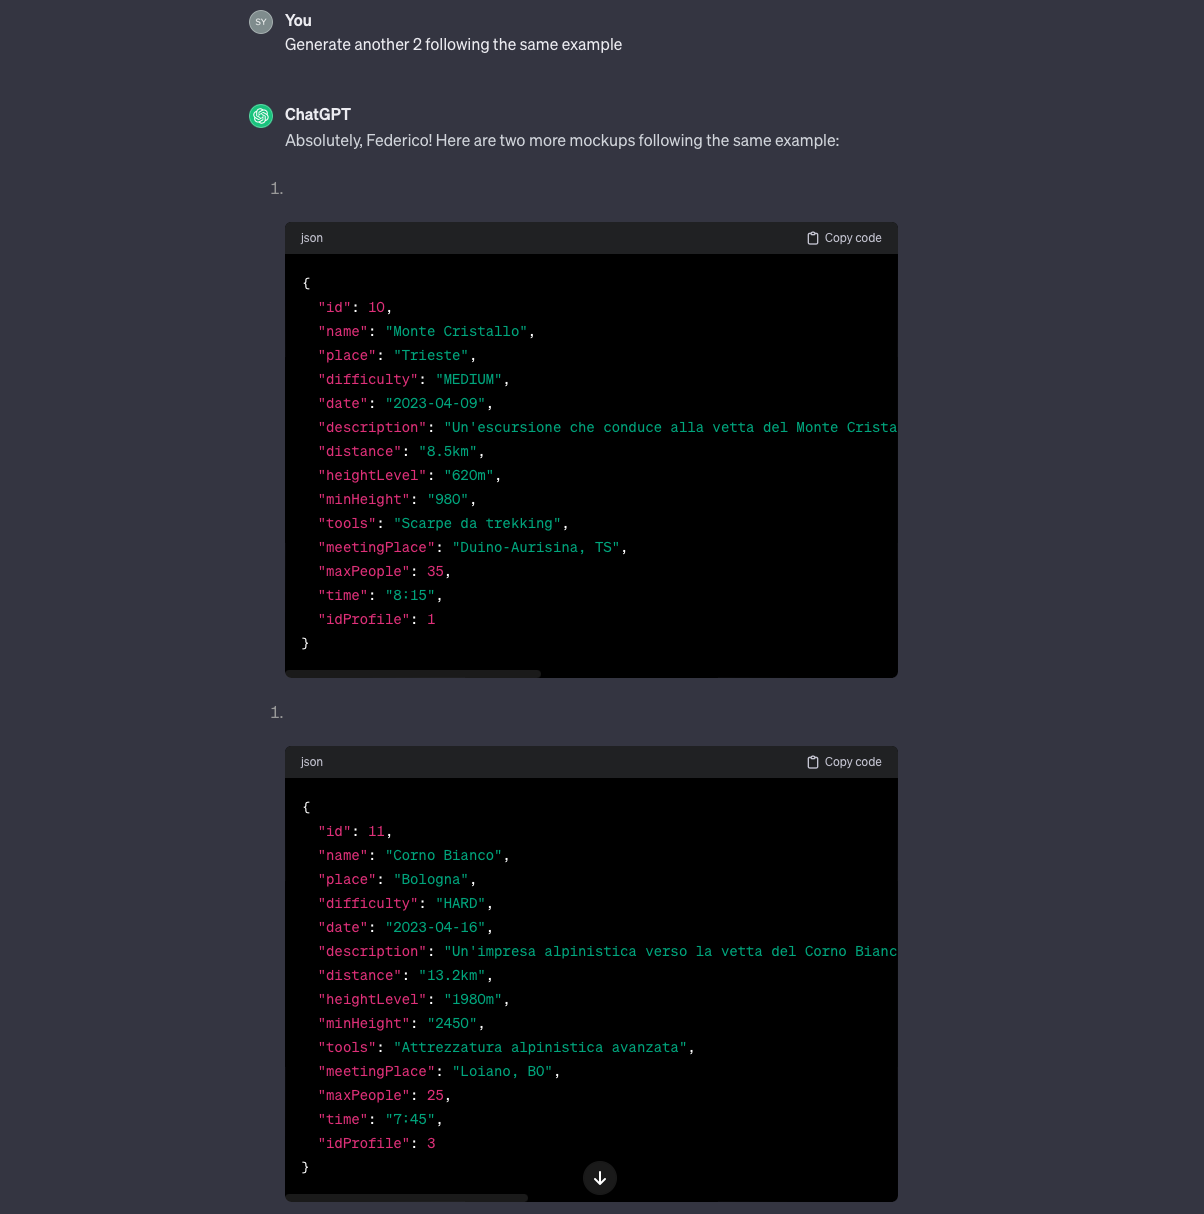
\includegraphics[width=\textwidth]{Iterazione 3/images/prompt2.png}
  \caption{Secondo prompt e risposta}\label{fig:prompt2}
\end{figure}
\begin{figure}[ht]
  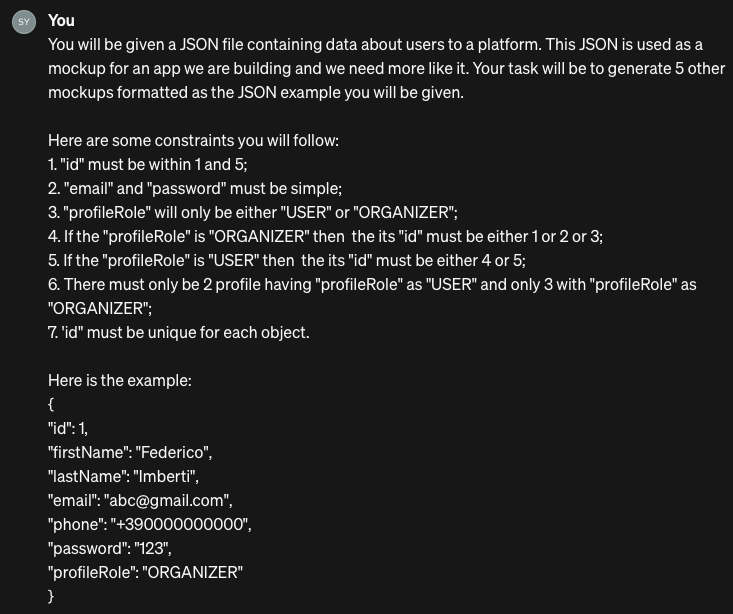
\includegraphics[width=\textwidth]{Iterazione 3/images/prompt3.png}
  \caption{Primo prompt per la generazione di utenti}\label{fig:prompt3}
\end{figure}
\begin{figure}[ht]
  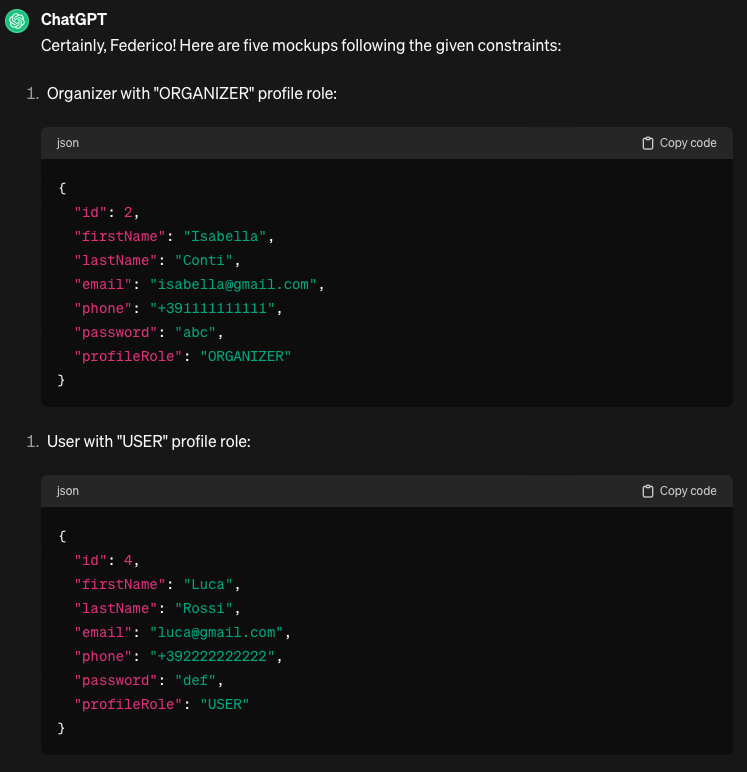
\includegraphics[width=\textwidth]{Iterazione 3/images/answer2.png}
  \caption{Risposta parziale al primo prompt}\label{fig:answ2}
\end{figure}
\begin{figure}[ht]
  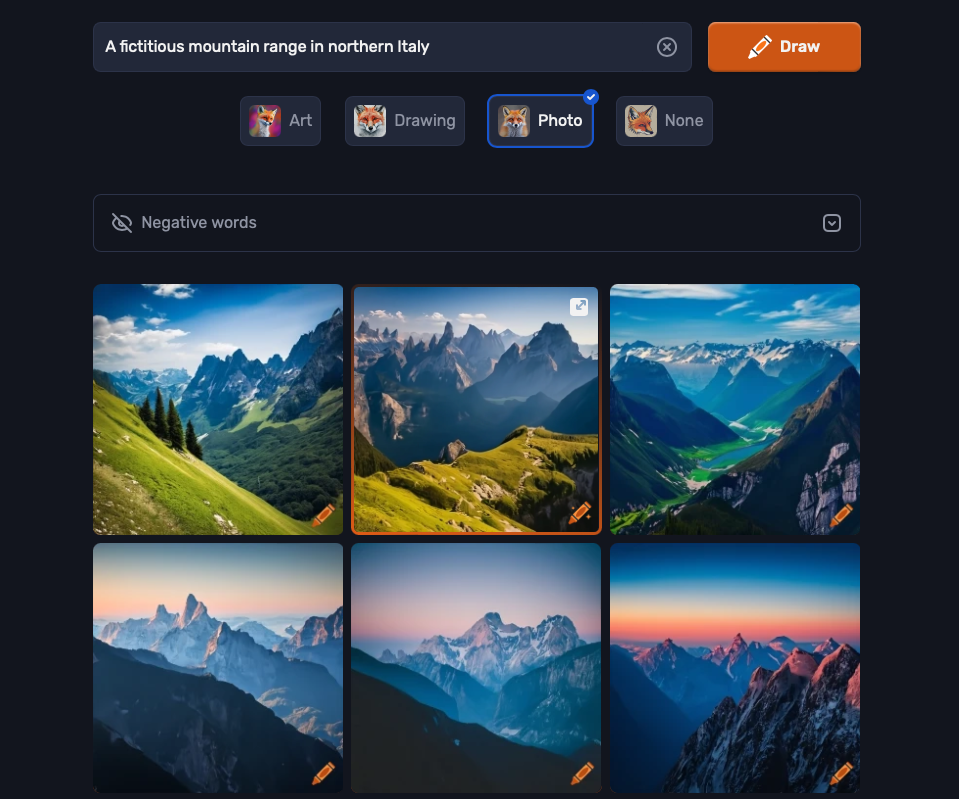
\includegraphics[width=\textwidth]{Iterazione 3/images/prompt4.png}
  \caption{Prompt per la generazione di immagini}\label{fig:prompt4}
\end{figure}